\documentclass[conference]{IEEEtran}
\IEEEoverridecommandlockouts

\usepackage{cite}
\usepackage{amsmath,amssymb,amsfonts}
\usepackage{algorithmic}
\usepackage{graphicx}
\usepackage{textcomp}
\usepackage{xcolor}
\def\BibTeX{{\rm B\kern-.05em{\sc i\kern-.025em b}\kern-.08em
    T\kern-.1667em\lower.7ex\hbox{E}\kern-.125emX}}
\begin{document}

\title{A Self-Healing Kalman Filter Framework for Multi-Robot Tracking in Indoor Service Environments\\}

\author{\IEEEauthorblockN{Yiğit YILMAZ}
\IEEEauthorblockA{\textit{Electrical Electronics Engineering Department} \\
\textit{Marmara University}\\
Istanbul, Turkiye \\
yigit.yilmaz@marun.edu.tr}
\and
\IEEEauthorblockN{Sıla Ilgıt KILINÇ}
\IEEEauthorblockA{\textit{Electrical Electronics Engineering Department} \\
\textit{Marmara University}\\
Istanbul, Turkiye \\
sila.ilgit@marun.edu.tr}
}

\maketitle

\begin{abstract}
Autonomous service robots are increasingly used in indoor environments such as restaurants, where reliable position tracking is essential for safe operation. However, tracking multiple robots becomes challenging when measurements are corrupted by noise or temporarily unavailable. This paper presents a multi-robot tracking framework based on Kalman filtering and evaluates its performance in a restaurant simulation developed in Webots. The system tracks multiple service robots using noisy position measurements and incorporates a self-healing mechanism that maintains state estimation during measurement outages. An Extended Kalman Filter (EKF) is also investigated for comparison with the standard Kalman Filter. Experimental results show that this Kalman-based approach reduces the tracking error by nearly 50\% compared to raw measurements. Furthermore, the self-healing mechanism maintains reliable tracking performance under measurement loss rates of approximately 15--17\%. The results demonstrate that this framework provides an effective and computationally efficient solution for indoor multi-robot tracking applications.
\end{abstract}

\begin{IEEEkeywords}
Kalman Filtering, Extended Kalman Filter, Multi-Target Tracking, Autonomous Mobile Robots, State Estimation, Measurement Loss Recovery, Indoor Navigation, Webots
\end{IEEEkeywords}

\section{Introduction}

Autonomous mobile robots are increasingly being deployed in indoor service environments such as restaurants, hospitals, warehouses, and shopping centers. In particular, restaurant service robots have gained significant attention due to their ability to improve operational efficiency, reduce workload, and provide contactless service. For these systems to operate safely and effectively, accurate tracking of robot positions is required at all times.

Reliable tracking in indoor environments remains a challenging problem \cite{thrun}. Sensor measurements are often corrupted by noise, while temporary communication failures or sensor outages may result in missing observations. These issues become even more critical when multiple robots operate simultaneously in the same environment \cite{multirobot}. as tracking errors may affect navigation performance and increase the risk of collisions.

State estimation techniques based on Kalman filtering have been widely used for target tracking and robot localization because of their computational efficiency and robustness against measurement noise \cite{kalman,welch,simon}. However, maintaining reliable estimates during measurement losses remains an important challenge in modern tracking systems \cite{tracking,barshalom}. Furthermore, nonlinear filtering approaches such as the Extended Kalman Filter (EKF) are frequently employed when the underlying system dynamics cannot be adequately represented by linear models \cite{ekf}.

This paper presents a multi-robot tracking framework designed for autonomous restaurant service robots. This system is evaluated in a Webots-based restaurant simulation and incorporates noisy position measurements, multi-target tracking, and a self-healing mechanism that enables state estimation to continue when measurements are temporarily unavailable. In addition, the performance of a standard Kalman Filter and an Extended Kalman Filter is compared under the same operating conditions.

The main contributions of this work can be summarized as follows:
\begin{itemize}
\item Development of a multi-robot tracking framework for restaurant service robots in a simulated indoor environment.
\item Implementation of a self-healing tracking mechanism capable of handling temporary measurement losses.
\item Comparative evaluation of Kalman Filter and Extended Kalman Filter approaches.
\item Performance assessment using RMSE-based tracking accuracy metrics.
\end{itemize}

\section{System Model}

\subsection{Restaurant Service Robot Scenario}

This tracking framework is evaluated in a restaurant service scenario developed in the Webots simulation environment \cite{webots}. The environment contains multiple service robots operating within an indoor restaurant area. The robots move between designated service locations while their positions are continuously monitored by a tracking system.

Two autonomous service robots are considered in this study. The robots follow predefined trajectories inside the restaurant environment and represent mobile agents responsible for food delivery tasks. To simulate realistic operating conditions, position measurements are corrupted by measurement noise. In addition, temporary measurement losses are introduced to evaluate the robustness of the self-healing tracking approach.

The objective of the tracking system is to estimate the positions of all robots as accurately as possible despite the presence of noisy and missing measurements.

\subsection{Process Model}

\begin{figure}[t]
\centering
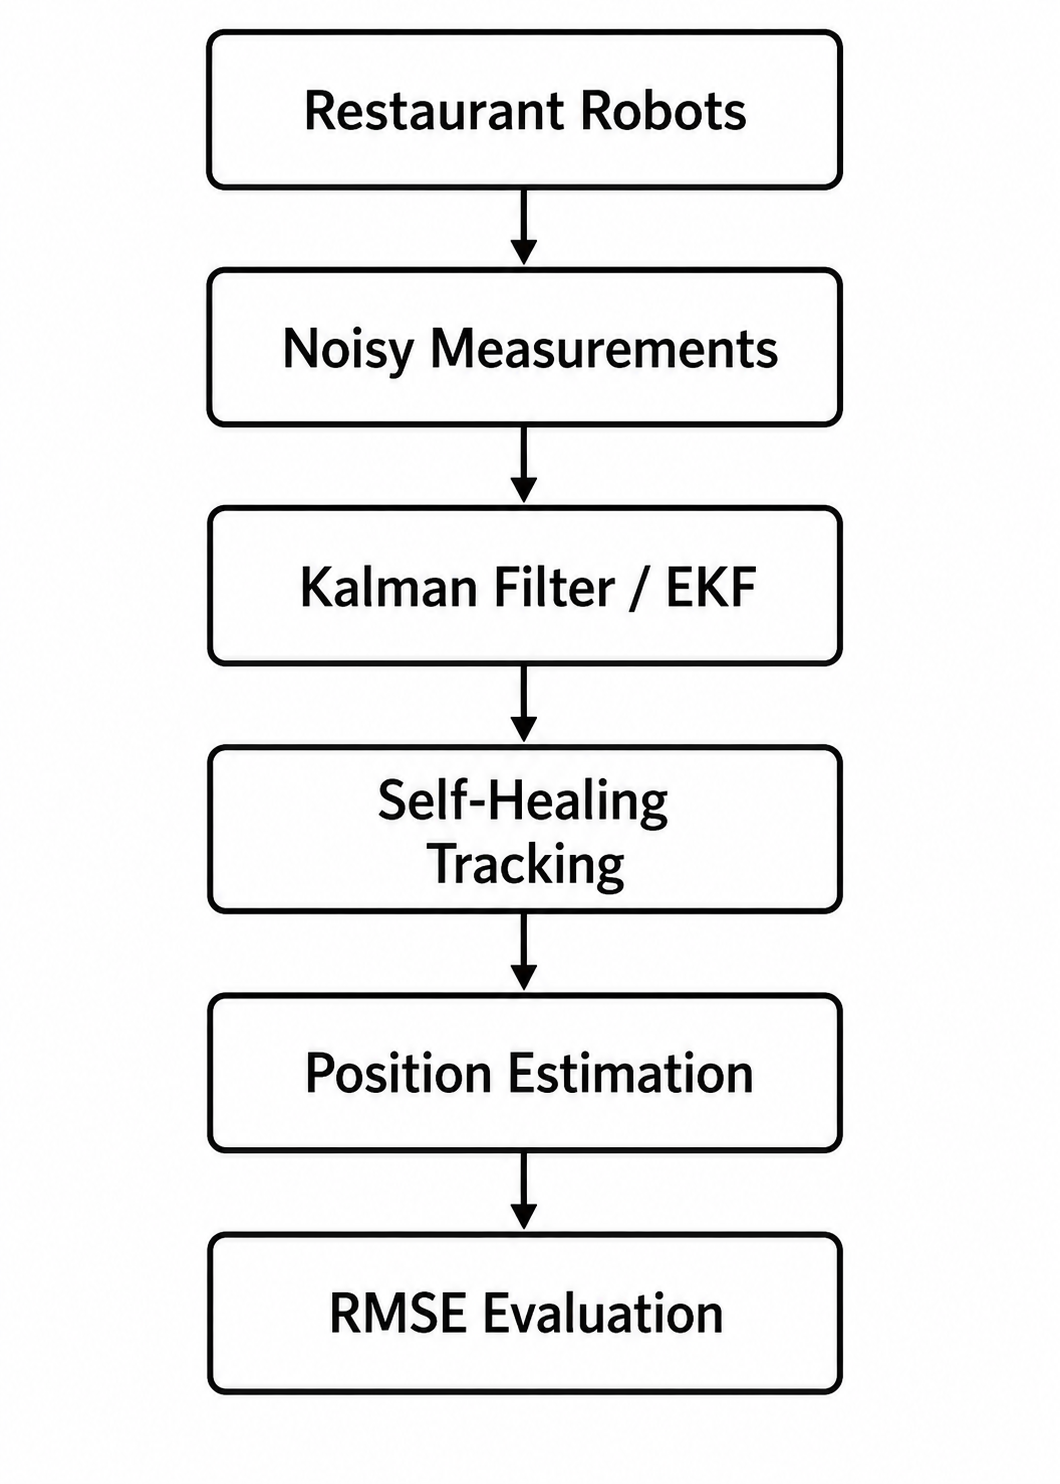
\includegraphics[width=\columnwidth]{System_diagram.png}
\caption{Overall process model of the tracking framework.}
\label{fig:process_model}
\end{figure}

The motion of each robot is represented using a constant-velocity state-space model. The state vector is defined as

\begin{equation}
\mathbf{x}_k=
\begin{bmatrix}
p_x\\
p_z\\
v_x\\
v_z
\end{bmatrix}
\end{equation}

where $p_x$ and $p_z$ denote the robot position coordinates and $v_x$ and $v_z$ represent the corresponding velocity components.

Assuming a constant velocity motion model, the state evolution can be expressed as

\begin{equation}
\mathbf{x}_k=
\mathbf{F}\mathbf{x}_{k-1}
+
\mathbf{w}_k
\end{equation}

where $\mathbf{w}_k$ denotes the process noise and

\begin{equation}
\mathbf{F}
=
\begin{bmatrix}
1 & 0 & \Delta t & 0\\
0 & 1 & 0 & \Delta t\\
0 & 0 & 1 & 0\\
0 & 0 & 0 & 1
\end{bmatrix}
\end{equation}

is the state transition matrix.

\subsection{Measurement Model}

The measurement system provides noisy observations of the robot positions. The measurement vector is defined as

\begin{equation}
\mathbf{z}_k=
\begin{bmatrix}
z_x\\
z_z
\end{bmatrix}
\end{equation}

where $z_x$ and $z_z$ are the measured position coordinates.

The measurement model is given by

\begin{equation}
\mathbf{z}_k
=
\mathbf{H}\mathbf{x}_k
+
\mathbf{v}_k
\end{equation}

where $\mathbf{v}_k$ denotes the measurement noise and

\begin{equation}
\mathbf{H}
=
\begin{bmatrix}
1 & 0 & 0 & 0\\
0 & 1 & 0 & 0
\end{bmatrix}
\end{equation}

is the observation matrix.

To emulate realistic sensor behavior, zero-mean random noise is added to the position measurements generated by the simulator.

\section{Filter Design}

\subsection{Kalman Filter}

The Kalman Filter (KF) is employed to estimate the position of each robot from noisy measurements \cite{kalman,welch}.. The filter operates recursively using two main stages: prediction and correction.

During the prediction stage, the state estimate and error covariance are propagated according to

\begin{equation}
\hat{x}_{k|k-1}=F\hat{x}_{k-1|k-1}
\end{equation}

\begin{equation}
P_{k|k-1}=FP_{k-1|k-1}F^T+Q
\end{equation}

where \(Q\) denotes the process noise covariance matrix.

When a new measurement becomes available, the filter performs the update step. The Kalman gain is computed as

\begin{equation}
K_k=P_{k|k-1}H^T(HP_{k|k-1}H^T+R)^{-1}
\end{equation}

where \(R\) is the measurement noise covariance matrix.

The state estimate is then updated according to

\begin{equation}
\hat{\mathbf{x}}_{k|k}
=
\hat{\mathbf{x}}_{k|k-1}
+
\mathbf{K}_k
\left(
\mathbf{z}_k
-
\mathbf{H}
\hat{\mathbf{x}}_{k|k-1}
\right)
\end{equation}

The Kalman Filter provides an efficient solution for estimating robot trajectories under noisy measurement conditions \cite{maybeck,simon}.

\subsection{Extended Kalman Filter}

In addition to the standard Kalman Filter, an Extended Kalman Filter (EKF) was implemented to investigate the effect of nonlinear motion modeling \cite{ekf}.

The EKF state vector is defined as

\begin{equation}
\mathbf{x}
=
\begin{bmatrix}
x\\
y\\
v\\
\theta
\end{bmatrix}
\end{equation}

where $x$ and $y$ denote the robot position, $v$ represents the linear velocity, and $\theta$ is the heading angle.

The nonlinear process model is expressed as

\begin{equation}
x_{k+1}
=
x_k
+
v_k \cos(\theta_k)\Delta t
\end{equation}

\begin{equation}
y_{k+1}
=
y_k
+
v_k \sin(\theta_k)\Delta t
\end{equation}

The EKF approximates the nonlinear system using first-order linearization through the Jacobian matrix \cite{ekf}. The resulting prediction and update procedures follow the standard EKF formulation.

The EKF was evaluated under the same simulation conditions as the standard Kalman Filter to compare tracking performance.

\subsection{Self-Healing Tracking Strategy}

A self-healing tracking mechanism was incorporated to improve robustness against temporary measurement losses. In practical indoor environments, communication interruptions or sensor failures may prevent measurements from being received at every sampling instant.

In this approach, when a measurement is unavailable, the filter continues operating using only the prediction stage. The update step is skipped until a valid measurement becomes available again.

Therefore, the state estimate evolves according to

\begin{equation}
\hat{\mathbf{x}}_k
=
\mathbf{F}
\hat{\mathbf{x}}_{k-1}
\end{equation}

during measurement outages.

This strategy enables continuous target tracking even when sensor data are temporarily missing. Once measurements become available again, the normal correction step is resumed. The self-healing mechanism allows the tracking system to maintain stable state estimates under intermittent measurement loss conditions.

\section{Experimental Setup}

\subsection{Simulation Environment}

The restaurant simulation environment used in this study is shown in Fig. 2. A restaurant-like indoor environment was created in Webots to evaluate this tracking framework. The environment consists of service robots, customer tables, and food serving locations. The robots move within the restaurant while noisy position measurements are collected for tracking purposes.

\begin{figure}[t]
\centering
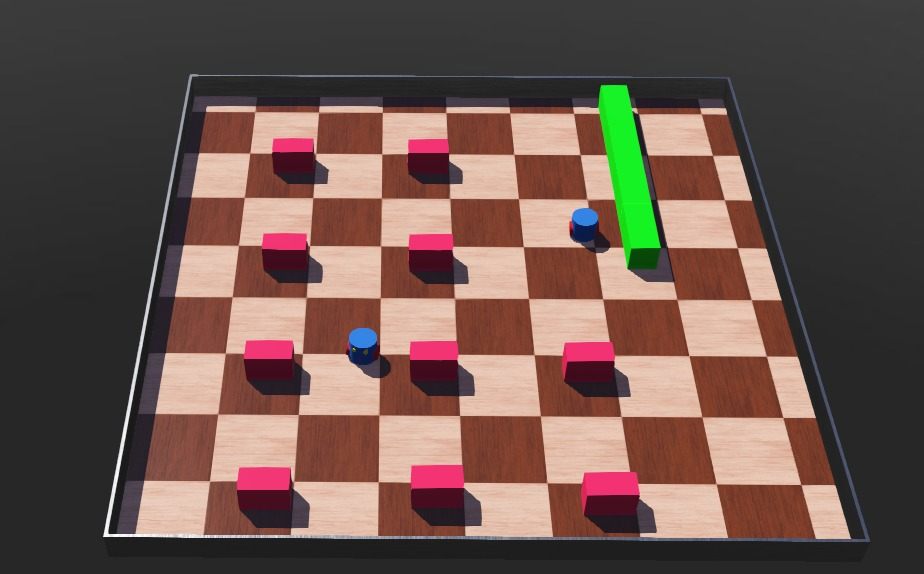
\includegraphics[width=\columnwidth]{restaurant_area.jpeg}
\caption{Restaurant simulation environment developed in Webots. The environment contains two service robots, ten customer tables, and food serving stations.}
\label{fig:restaurant_environment}
\end{figure}

\subsection{Simulation Parameters}

\begin{table}[h]
\caption{Simulation Parameters}
\centering
\begin{tabular}{|c|c|}
\hline
Parameter & Value\\
\hline
Arena Size & 2m x 2m\\
Number of Robots & 2\\
Number of Tables & 10\\
Measurement Noise & 0.02 m\\
Time Step & 64 ms\\
Measurement Loss Rate & 15-17\%\\
\hline
\end{tabular}
\end{table}

The simulation was executed using a sampling period of 64 ms. Position measurements were corrupted by uniformly distributed random noise with a maximum amplitude of approximately 0.02 m. Two service robots were tracked simultaneously throughout the simulation.

To evaluate robustness against missing measurements, random measurement losses were introduced during the self-healing experiments. Approximately 15--17\% of the measurements were intentionally removed to simulate temporary sensor outages or communication interruptions.

The generated tracking data were stored in CSV format and processed offline using Python-based implementations of the tracking algorithms.

\subsection{Performance Metric}

Tracking performance was evaluated using the Root Mean Square Error (RMSE), which is commonly used in target tracking applications \cite{tracking}. Between the estimated robot positions and the corresponding ground-truth positions obtained from the simulator.

The RMSE is defined as

\begin{equation}
RMSE =
\sqrt{
\frac{1}{N}
\sum_{k=1}^{N}
\left(
(x_k-\hat{x}_k)^2
+
(y_k-\hat{y}_k)^2
\right)
}
\end{equation}

where $(x_k,y_k)$ represents the true robot position and $(\hat{x}_k,\hat{y}_k)$ denotes the estimated position at time step $k$.

A lower RMSE value indicates a more accurate tracking performance. The same metric was used to compare the raw measurements, the Kalman Filter estimates, the Extended Kalman Filter estimates, and the Self-Healing tracking results. 



\section{Results and Discussion}

\subsection{Kalman Filter Performance}



Table~\ref{tab:kf_results} presents the tracking performance of the standard Kalman Filter for both service robots.

\begin{table}[h]
\centering
\caption{Kalman Filter Tracking Performance}
\label{tab:kf_results}
\resizebox{\columnwidth}{!}{
\begin{tabular}{|c|c|c|}
\hline
Target & Measurement RMSE (m) & Kalman RMSE (m) \\
\hline
TARGET\_1 & 0.0117 & 0.0060 \\
TARGET\_2 & 0.0115 & 0.0059 \\
\hline
\end{tabular}}
\end{table}

The Kalman Filter significantly improved tracking accuracy for both robots. For TARGET\_1, the RMSE was reduced from 0.0117 m to 0.0060 m, while for TARGET\_2 the error decreased from 0.0115 m to 0.0059 m. These results correspond to an error reduction of approximately 49\%, demonstrating the effectiveness of Kalman filtering in suppressing measurement noise.

\begin{figure}[t]
\centering
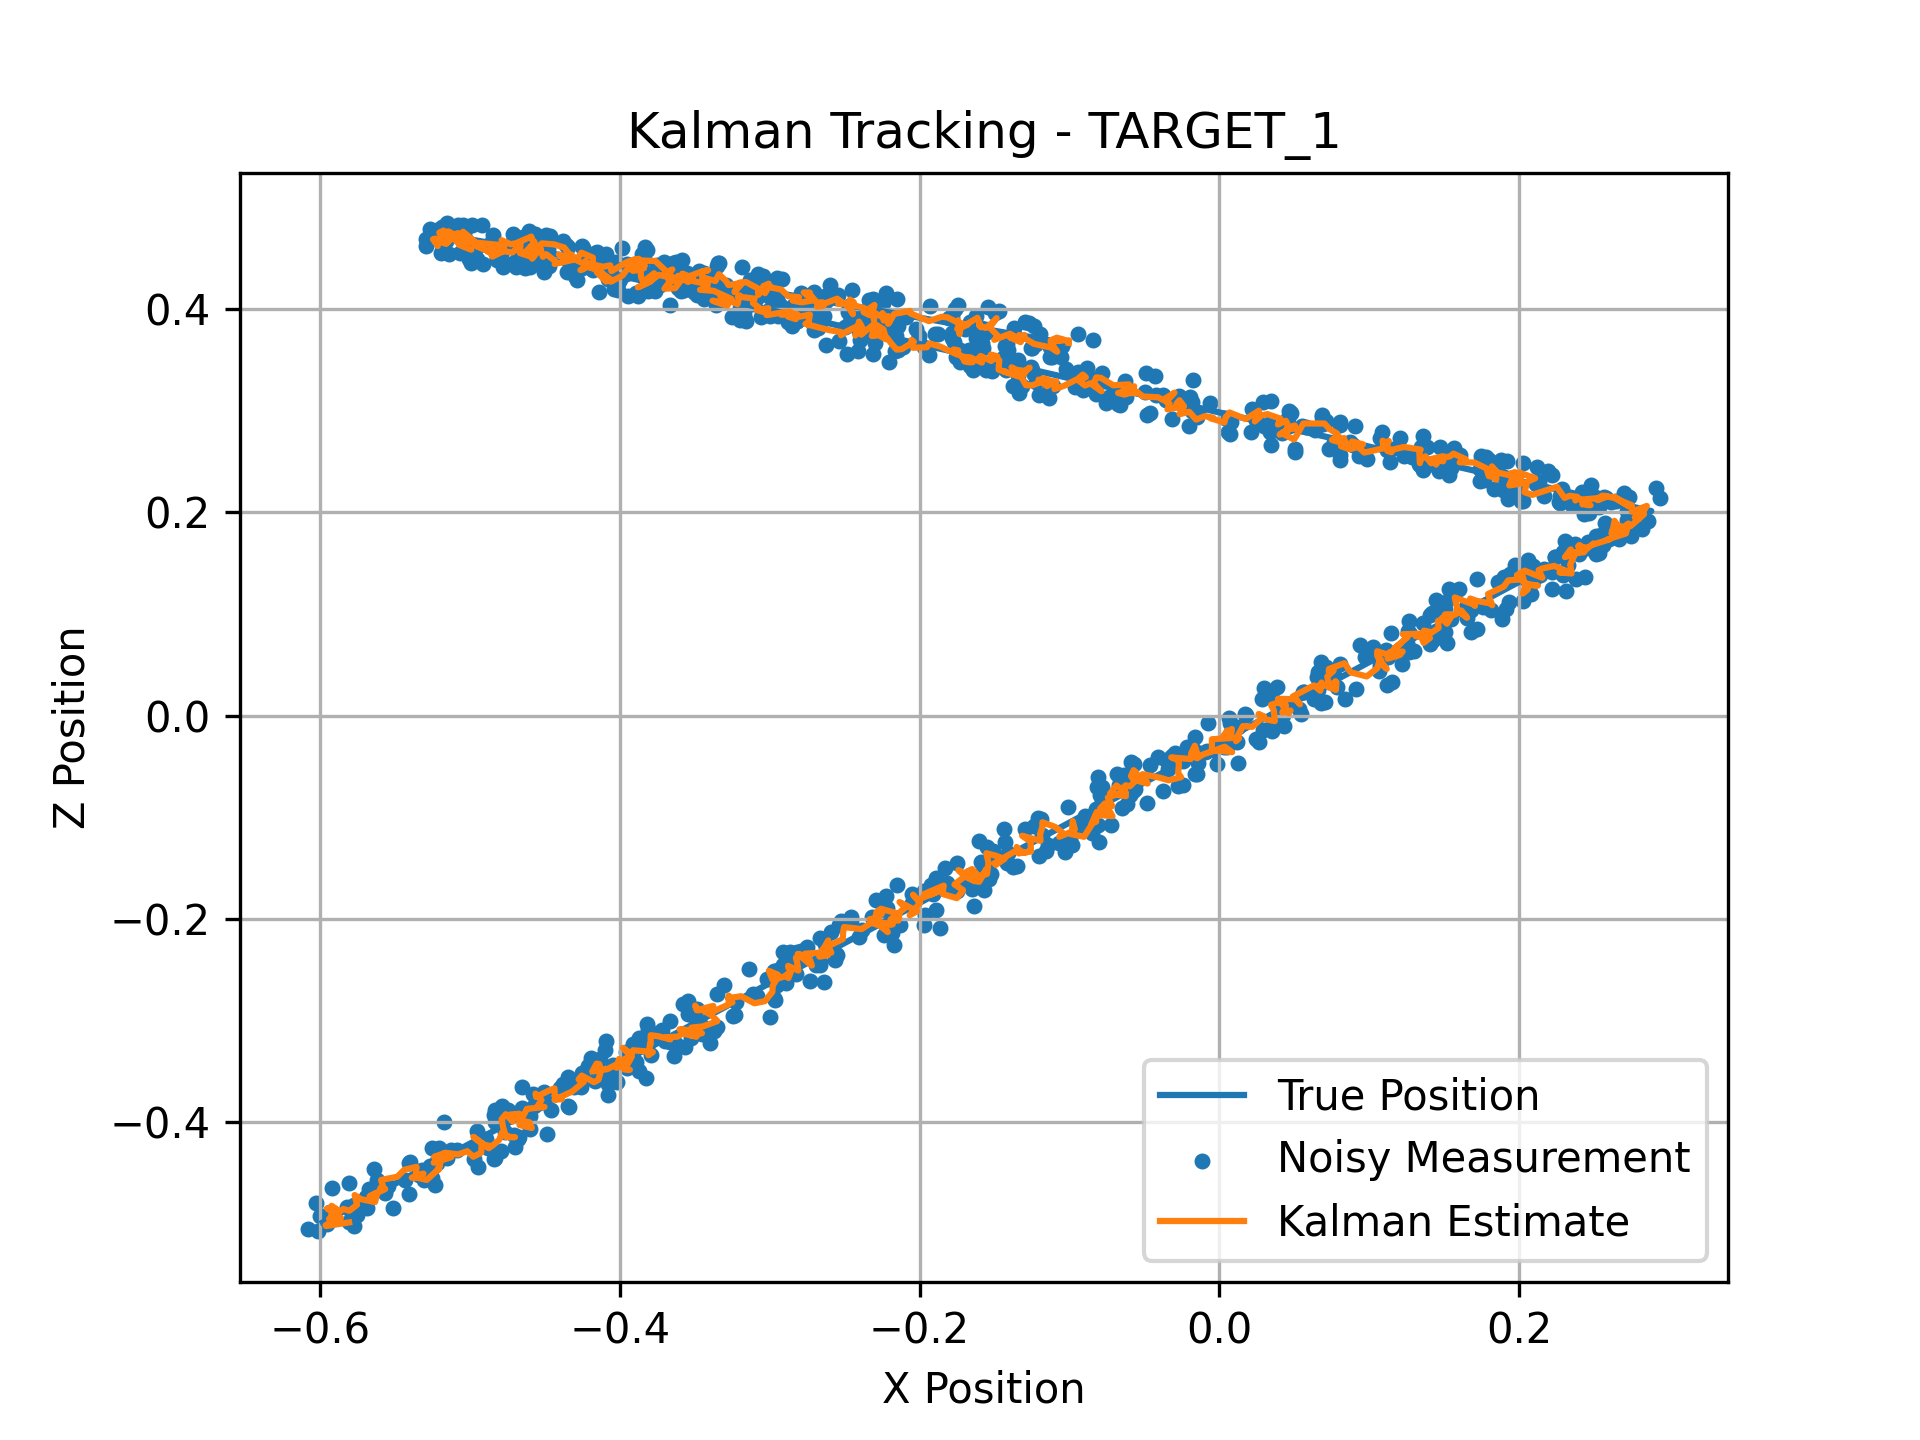
\includegraphics[width=\columnwidth]{TARGET_1_kalman_plot.png}
\caption{Tracking performance of the Kalman Filter for TARGET\_1. The estimated trajectory closely follows the true trajectory while reducing measurement noise.}
\label{fig:kf_tracking}
\end{figure}

The obtained results indicate that the Kalman Filter reduced the tracking error by nearly 50\% for both robots compared to the raw noisy measurements.

\subsection{Self-Healing Tracking Performance}

The self-healing tracking mechanism was evaluated under randomly generated measurement losses.

\begin{table}[h]
\centering
\caption{Self-Healing Tracking Results}
\label{tab:self_healing}
\resizebox{\columnwidth}{!}{
\begin{tabular}{|c|c|c|c|}
\hline
Target & Loss Rate (\%) & Measurement RMSE (m) & Self-Healing RMSE (m) \\
\hline
TARGET\_1 & 16.67 & 0.0117 & 0.0065 \\
TARGET\_2 & 15.51 & 0.0114 & 0.0062 \\
\hline
\end{tabular}}
\end{table}

Despite the loss of approximately 15--17\% of the measurements, the self-healing mechanism maintained stable tracking performance. The resulting estimation errors remained close to those obtained with complete measurements, indicating that the prediction stage of the filter successfully compensated for temporary measurement outages. This demonstrates that this framework can continue providing reliable position estimates even when sensor data becomes temporarily unavailable.

\begin{figure}[t]
\centering
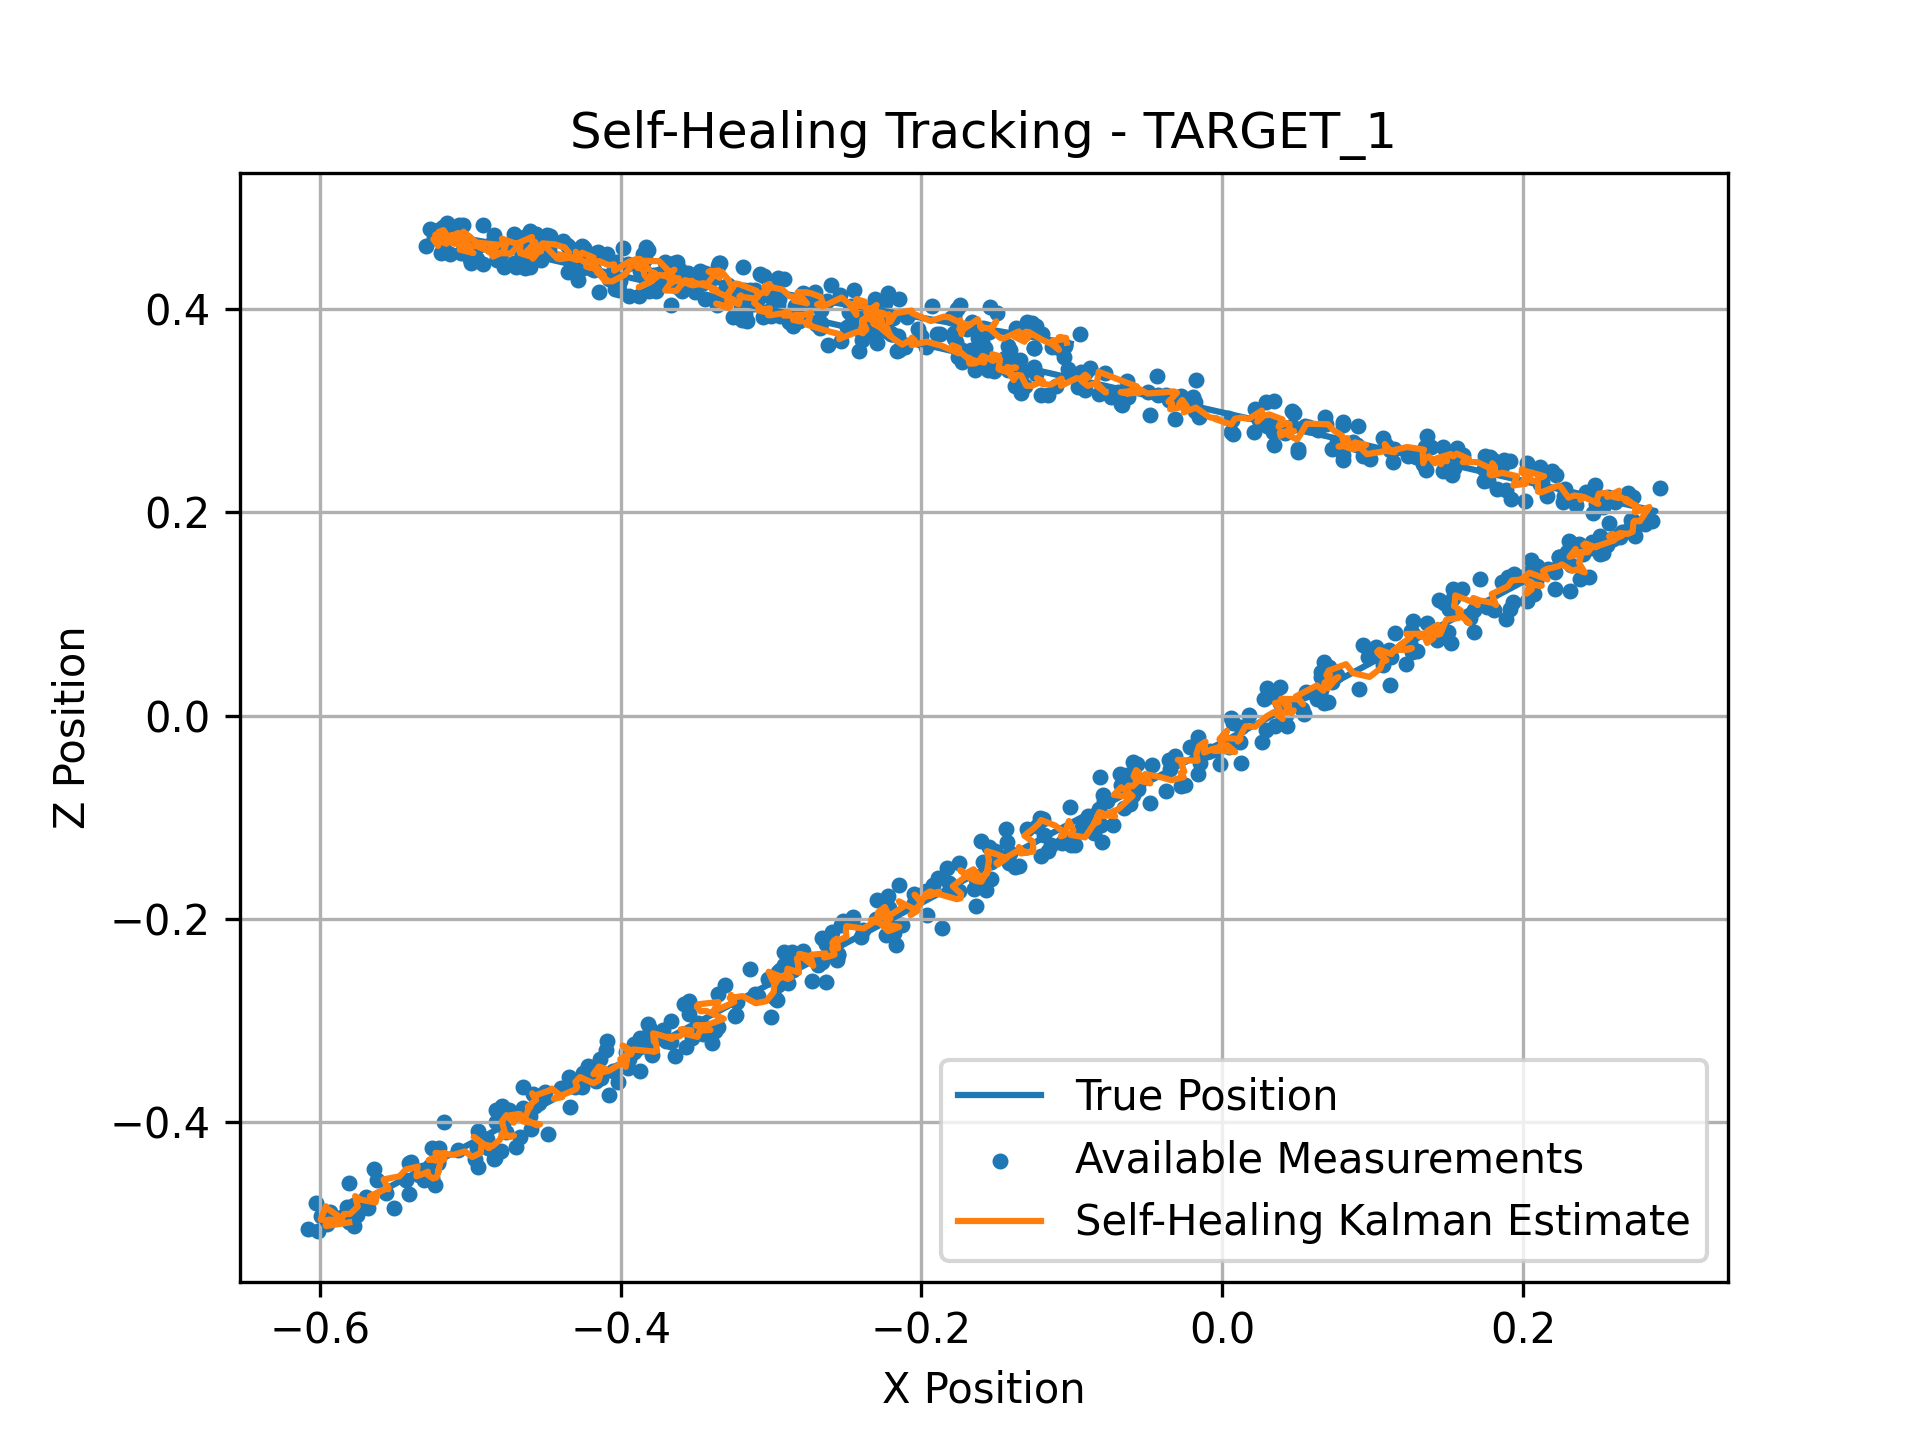
\includegraphics[width=\columnwidth]{TARGET_1_self_healing_plot.png}
\caption{Self-healing tracking results for TARGET\_1. The filter maintains trajectory estimation despite temporary measurement losses.}
\label{fig:selfhealing_tracking}
\end{figure}


\subsection{EKF Comparison}

\begin{figure}[t]
\centering
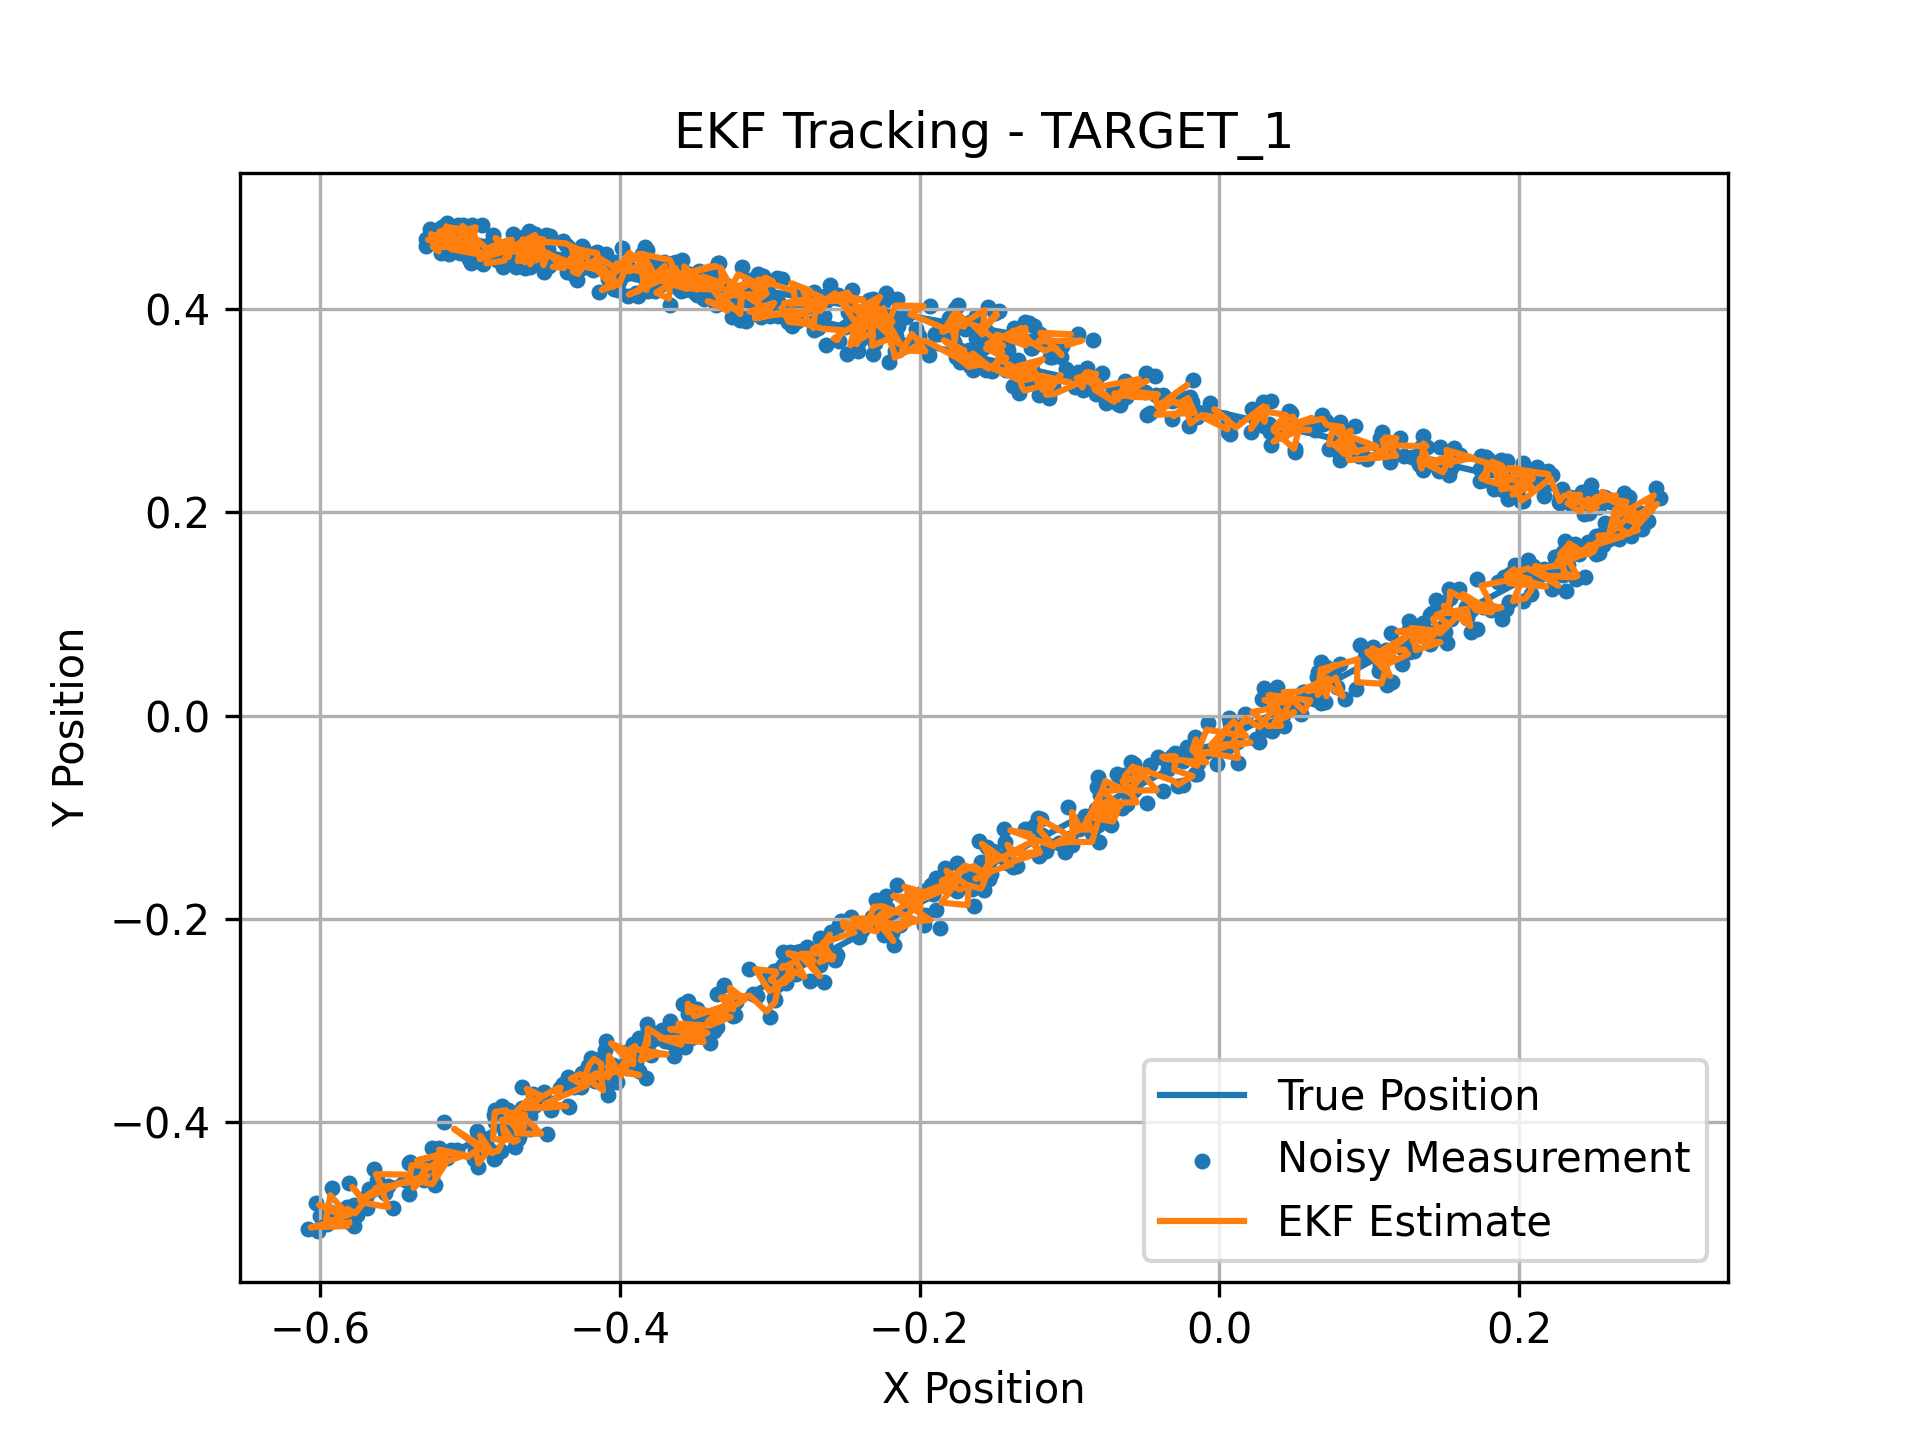
\includegraphics[width=\columnwidth]{TARGET_1_ekf_plot.png}
\caption{EKF tracking performance for TARGET\_1.}
\label{fig:ekf_tracking}
\end{figure}

A comparison between the standard Kalman Filter and the Extended Kalman Filter is presented in Table~\ref{tab:ekf_comparison}.

\begin{table}[h]
\centering
\caption{Kalman Filter and EKF Comparison}
\label{tab:ekf_comparison}
\resizebox{\columnwidth}{!}{
\begin{tabular}{|c|c|c|c|}
\hline
Target & Measurement RMSE (m) & KF RMSE (m) & EKF RMSE (m) \\
\hline
TARGET\_1 & 0.0117 & 0.0060 & 0.0095 \\
TARGET\_2 & 0.0115 & 0.0059 & 0.0092 \\
\hline
\end{tabular}}
\end{table}

The Extended Kalman Filter also improved the tracking accuracy compared to raw measurements. However, the standard Kalman Filter achieved lower RMSE values in both tracking scenarios. This behavior can be explained by the predominantly linear motion of the robots in the simulation environment. Since the robot trajectories closely followed a constant-velocity model, the additional nonlinear modeling capability of the EKF did not provide a significant advantage. Therefore, the additional computational complexity of the EKF was not justified for the considered tracking scenario. In addition, the EKF introduces linearization errors through Jacobian-based approximations. Since the simulated trajectories did not exhibit strong nonlinear behavior, the additional model complexity did not improve estimation performance.

\begin{table}[h]
\centering
\caption{Overall Performance Comparison}
\label{tab:overall_comparison}
\begin{tabular}{|c|c|c|c|}
\hline
Method & TARGET\_1 & TARGET\_2 & Average \\
\hline
Measurements & 0.0117 & 0.0115 & 0.0116 \\
Kalman Filter & 0.0060 & 0.0059 & 0.0060 \\
Self-Healing KF & 0.0065 & 0.0062 & 0.0064 \\
EKF & 0.0095 & 0.0092 & 0.0094 \\
\hline
\end{tabular}
\end{table}

Table V summarizes the overall performance of all evaluated methods. The standard Kalman Filter achieved the lowest average RMSE, while the self-healing approach maintained comparable accuracy despite measurement losses. The EKF improved over raw measurements but did not outperform the linear Kalman Filter in this scenario.

\section{Conclusion}

This paper presented a multi-robot tracking framework for autonomous service robots operating in an indoor restaurant environment. This approach combines Kalman filtering, self-healing tracking, and Extended Kalman Filter (EKF) techniques to estimate robot positions from noisy measurements.

A restaurant scenario was developed in the Webots simulation environment, where multiple service robots were tracked using position measurements affected by random noise. Experimental results demonstrated that the standard Kalman Filter significantly improved tracking accuracy, reducing the position estimation error by approximately 49\% compared to raw measurements. In addition, the tested self-healing mechanism successfully maintained reliable tracking performance even when approximately 15--17\% of the measurements were unavailable.

The Extended Kalman Filter was also evaluated and was found to improve the tracking accuracy compared to raw measurements. However, the standard Kalman Filter achieved lower estimation errors due to the predominantly linear motion characteristics of the simulated robot trajectories.

Overall, the results indicate that this framework provides an effective and computationally efficient solution for indoor multi-robot tracking applications. Future work may include obstacle-aware path planning, cooperative multi-robot coordination, and the integration of additional sensors such as LiDAR and cameras for enhanced localization performance.


\section*{Acknowledgement}

The authors acknowledge the use of ChatGPT to assist in generating initial drafts of selected sections of the manuscript and Python scripts used during the experimental evaluation. All generated content was reviewed, tested, and verified by the authors.

\section*{}

\bibliographystyle{IEEEtran}
\bibliography{references}

\end{document}